\input{common/onetextpage.tex}
\newcounter{nappendix}
\renewcommand{\thenappendix}{\Alph{nappendix}}
\newcommand{\newappendix}[1]{%
    \addtocounter{chapter}{1}
    \refstepcounter{nappendix}
    \onetextpage{Appendix \thenappendix}
    \chapter*{Appendix \thenappendix: #1}
    \label{appendix:\thenappendix}
    \addcontentsline{toc}{chapter}{Appendix \thenappendix: #1}
    \renewcommand{\thesection}{\thenappendix.\arabic{section}}
    \renewcommand{\thesubsection}{\thesection.\arabic{subsection}}
    \renewcommand{\thefigure}{\thenappendix.\arabic{figure}}
    \setcounter{figure}{0}
    \setcounter{section}{0}
}

\newappendix{Recommendation Engine}
% Because it's too long, so we need a place to describe everything.
This appendix chapter describes KU Eater's recommendation engine and the steps to reach the end goal.

\section{Fine-tuning our language model to understand food \& ingredients}
\label{section:finetune-lm}
This step is where we need to create an embedding model to encode textual ingredients and dish names into our vector store.
Moreover, KU Eater's primary nature is to cater to all students in Kasetsart University, there are a few requirements for our embedding model:

\textbf{(1)} Our embedding model needs to support at least English and Thai language, \textbf{(2)} Our embedding model needs to be lightweight and fast to load,
and \textbf{(3)} Our embedding model needs to be easily maintainable.

We found "WangchanBERTa\cite{lowphansirikul2021wangchanberta}" an English and Thai embedding model, meeting our first requirement.
The model has a size of 106 million parameters and a sparse vector size of 768, which in theory, is easy to load on medium machines with low-end
graphics adapter; thus, satisfying our second requirement. However for the third criterion, it is up to us to build a pipeline that will
update and maintain the embedding model once in a while.

We need to feed information on ingredients and dishes for the base model to learn, this is called "Fine-tuning." For now, our model will learn
the information on ingredients, the methodology consists of (1) turning data from structured object pairs e.g.,

\begin{verbatim}
    # Sample ingredient objects

    ingredient_name: "Fish sauce",
    category: "Condiment",
    allergen_groups: ["fish"],
    similar_ingredients: ["Soy sauce",]

    ingredient_name: "Soy sauce",
    category: "Condiment",
    allergen_groups: ["soy", "gluten"],
    similar_ingredients: ["Fish sauce",]

    ingredient_name: "Ketchup",
    category: "Condiment",
    allergen_groups: ["gluten"],
    similar_ingredients: ["Chili sauce"]

    ####

    # Turn into texts,
    "Fish sauce: a Condiment with allergen group of fish,
    similar to Soy sauce,"
    "Soy sauce: a Condiment with allergen group of soy,
    gluten, similar to Fish sauce,"
    "Ketchup: a Condiment with allergen group of gluten,
    similar to Chili sauce,"
\end{verbatim}

The texts are used to fit into the base model, allowing the model to understand more context on what the ingredient names meant. Then,
(2) we reinforce our model to learn the relation of items, we cluster the categories of ingredients to be separated groups. In each group then
perform a Contrastive learning using Triplets. It is a method to make our model distance some vectors that are uncorrelated to each other, e.g.,

\begin{verbatim}
    # The format of a triplet is: (anchor, positive, negative)

    # We know that fish sauce & soy sauce has high similarity
    # but ketchup is a different condiment from the two,
    # the triplet is:
    (fish sauce, soy sauce, ketchup)
    # or,
    (soy sauce, fish sauce, ketchup)
    # for ketchup training,
    (ketchup, chili sauce, fish sauce)
\end{verbatim}

Lastly, (3) we can implement functions to see ingredient similarity,
identify allergen groups an ingredient has etc.

For the menu items (dishes) we can pass textual context into the model to fit, for example,
"Rice with crispy pork and holy basil: a dish from stall Nong Pim A LA CARTE (Stir Fry),
it contains Rice, Crispy pork, Holy basil, Chili, Garlic, Fish sauce, Soy sauce, oil,"

The entire process of finetuning is found at \url{https://colab.research.google.com/drive/1WWwTQFG3dHQORTU20ZimSLLUgdgs9GE_?usp=sharing}.

\section{Designing a recommendation engine}
This step is the design process of KU Eater's recommendation engine,
it bases itself using the embedding model from \ref{section:finetune-lm}.

\subsection{Preliminary Step: Populate KU Eater's database with embeddings vectors}
Using the embedding model from last step, we can pipeline our dish names,
ingredients and stalls from our database into it to retrieve list of vectors.

Then the vectors must be put in respective places inside our database, for example,
in the MenuItem table, there must be both menu name and its generated embedding;
or in the Ingredient table, an embedding vector must occupy an ingredient entry.

\subsection{Usage 1: Finding dishes with similar names}
We can implement a function that reads from user profiles, to see what dishes they liked.

From the liked dishes, the recommendation engine will select a number of dishes
to be anchor dish---meaning, any recommended dish must have similar name to the anchor dish.

For each anchor dish, we can use its embedding vector to
find menu items closest to it.

\subsection{Usage 2: Finding dishes with similar ingredients}
We can implement a function that reads from user profiles, to see what dishes they liked.

From the liked dishes, the recommendation engine will select a number of dishes
to be anchor dish---meaning, any recommended dish must have some ingredients as same as the anchor.

For each anchor dish, it should be a point in our vector space, so we can perform
K-nearest neighbors to retrieve a list of dishes that are near (similar) to the anchor dish.
This is a content-based filtering process.

\subsection{Final Step: Scoring system}
KU Eater has a final component of scoring dishes based on user preferences
before the recommendations get shown to the users. The following is the breakdown of
how scoring is considered:

\begin{figure}[h!]
    \centering
    \includesvg[width=\textwidth,height=0.2\textheight,keepaspectratio]{kueater/algo_prediction.svg}
    \caption{Pipeline for Predicting Recommendations}
    \label{fig:pipeline-for-predicting-2}
\end{figure}

\begin{itemize}[leftmargin=80pt]
    \item If the dish contains allergens linked to user profile, it is \textbf{discarded}.
    \item If the dish contains ingredients that constitutes dietary restrictions, it is \textbf{discarded}.
    \item Any liked dishes gets recommended, \textbf{increase} score.
    \item Any dishes from liked stall gets recommended, \textbf{increase} score.
    \item Any disliked dishes gets recommended, \textbf{decrease} score.
    \item Any dishes contain disliked ingredients gets recommended, \textbf{decrease} score. (Not done within the timeframe)
\end{itemize}

\subsection{Evaluating the recommendation engine}
\label{subsection:recsys-eval}
The embedding model that was finetuned using our data is evaluated using a binary classification technique.
The same-formatted sentences which are unseen by training process\footnote{\url{https://huggingface.co/datasets/GToidZ/kueater-test-set}}
are fed into the model to be predicted. As a result, the model has the following performance metrics:

\begin{itemize}[leftmargin=80pt]
    \item The model achieves an accuracy of \textbf{64.72\%} which is a moderate model and has room for improvement.
    \item Precision is moderate with value of \textbf{64.77\%} indicating that the model can generate false positives.
    \item Recall is very high at \textbf{99.36\%} indicating that the model is liberal at capturing the true positives correctly.
    \item F1 score is higher than the model's accuracy at, \textbf{78.42\%} reflecting that the model needs further improvements.
\end{itemize}

The results above suggests that the model classes are likely imbalanced and needs further refinement in the next revisions.

We certainly think that metrics and scoring can potentially lead us in
the right way within the development phase, but in order to evaluate
whether the recommendation system is working as intended is by gathering
user feedback and retention. Including performing questionnaire when user
is using the application.

\subsection{Commentary from the author}
We think that our model did not do well enough in the end. There are 
inconsistencies and inaccurate predictions. We thought that the model
does not train on data well fitted enough, or has little to no feature that
we started to generate some numbers (e.g. Diet Compatibility).

We also tried to include tagging into our model but it resulted in model being
too overconfidence that it tagged items in our model incorrectly. We also think that
the problem probably lies in the base model that we used, with it being trained
on Wikipedia data, we suspect that the model can be too general and that
results in us needing to have more data with more features.

\newappendix{Application Screen Samples}
In this appendix, redirected from \ref{chap:deliverable}, presents the screenshot samples of KU Eater.

\begin{figure}[h!]
    \centering
    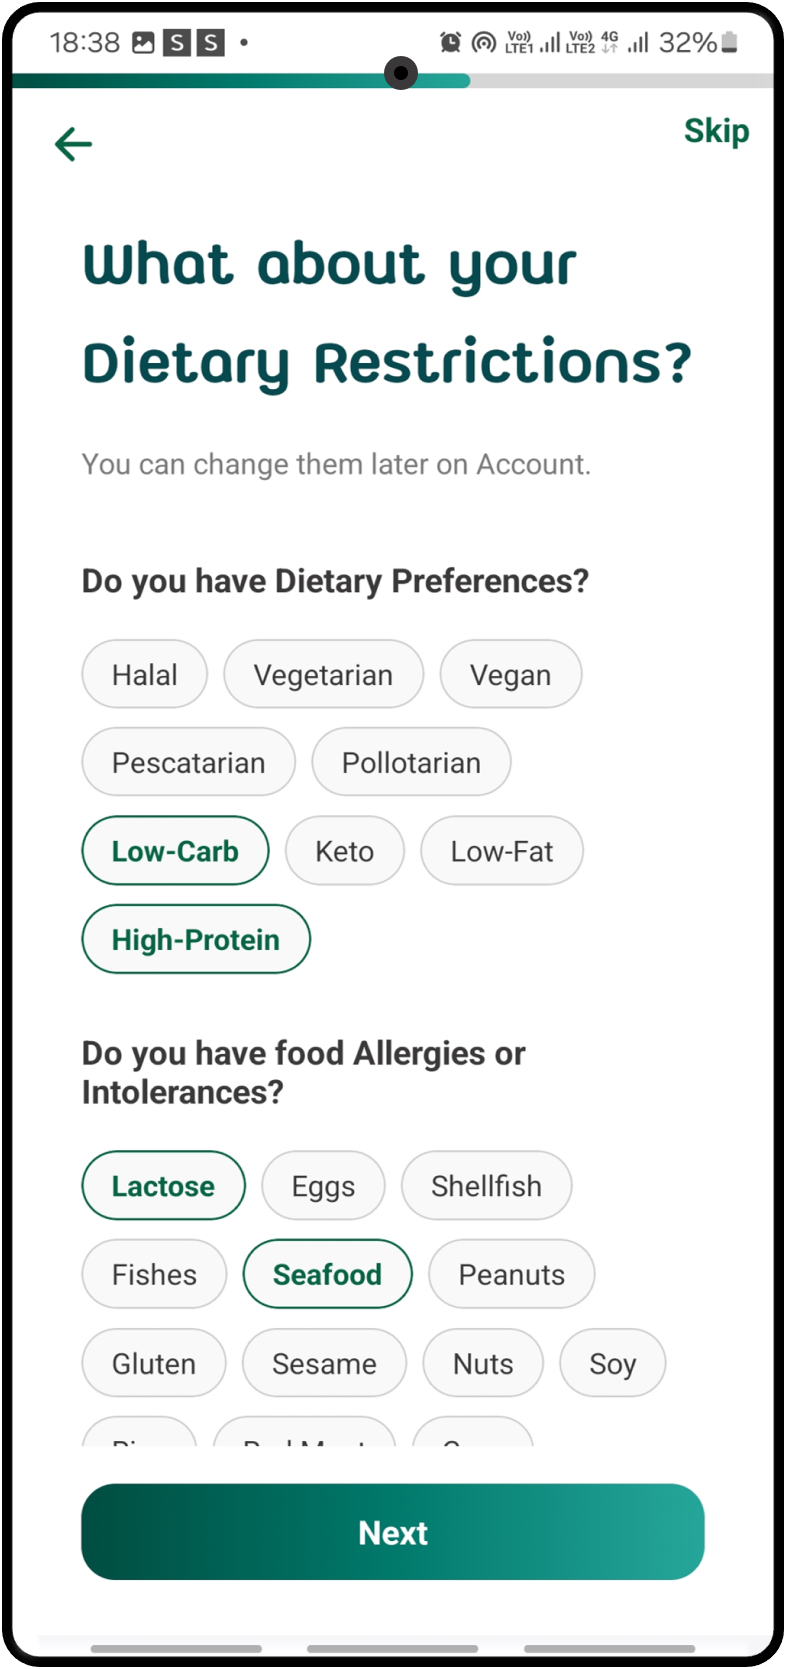
\includegraphics[width=\textwidth,height=0.4\textheight,keepaspectratio]{kueater/screenshots/dietary-restrictions.png}
    \caption{Dietary Restrictions}
    \label{fig:dietary-restrictions-screen}
\end{figure}

\begin{figure}[h!]
    \centering
    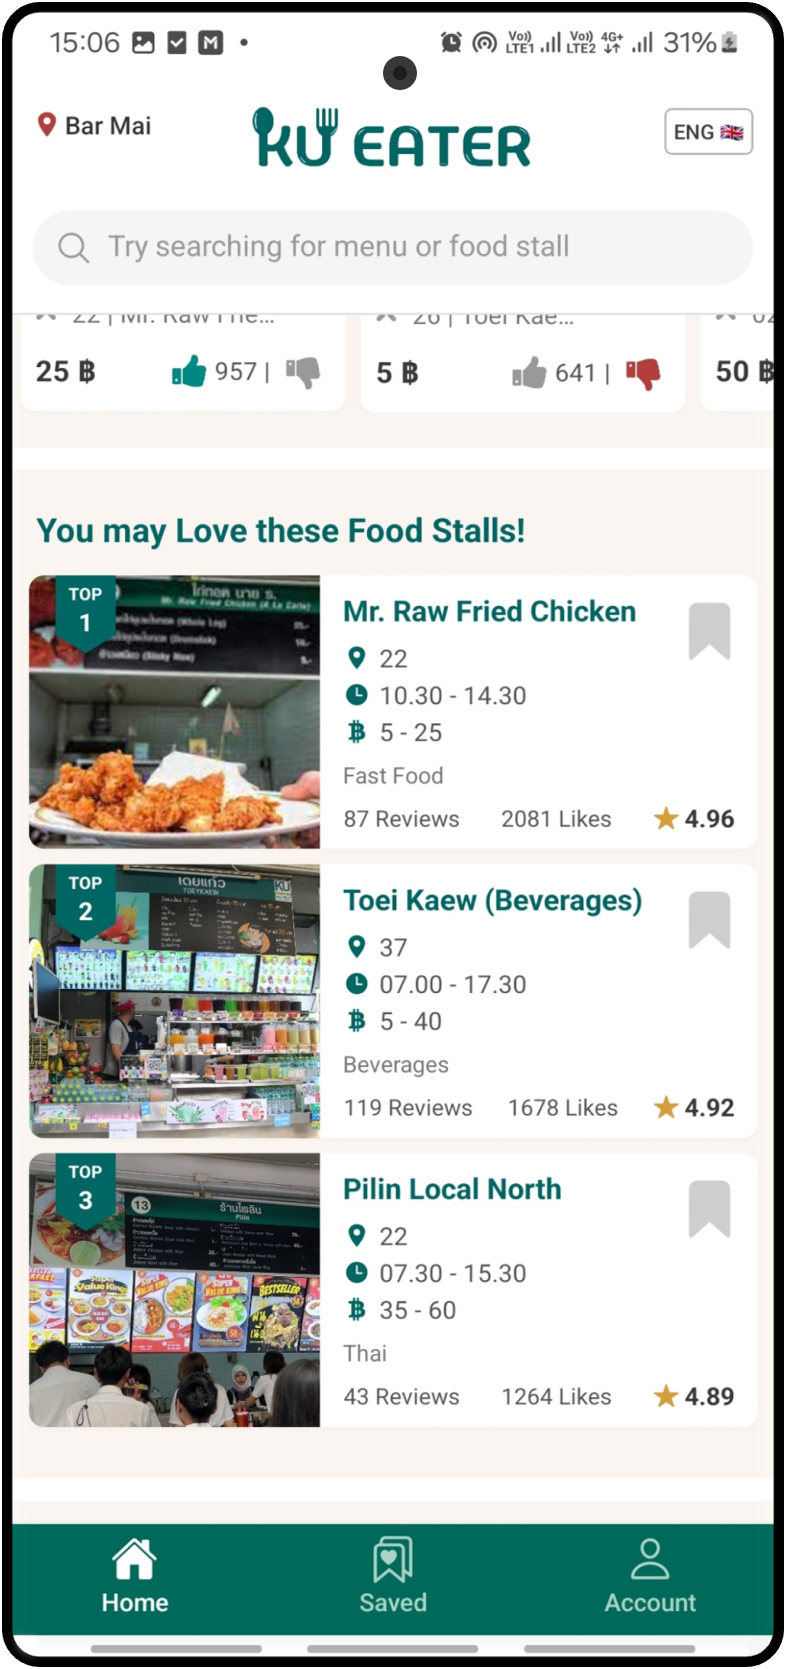
\includegraphics[width=\textwidth,height=0.4\textheight,keepaspectratio]{kueater/screenshots/home-screen.png}
    \caption{Home Screen}
    \label{fig:home-screen}
\end{figure}

\begin{figure}[h!]
    \centering
    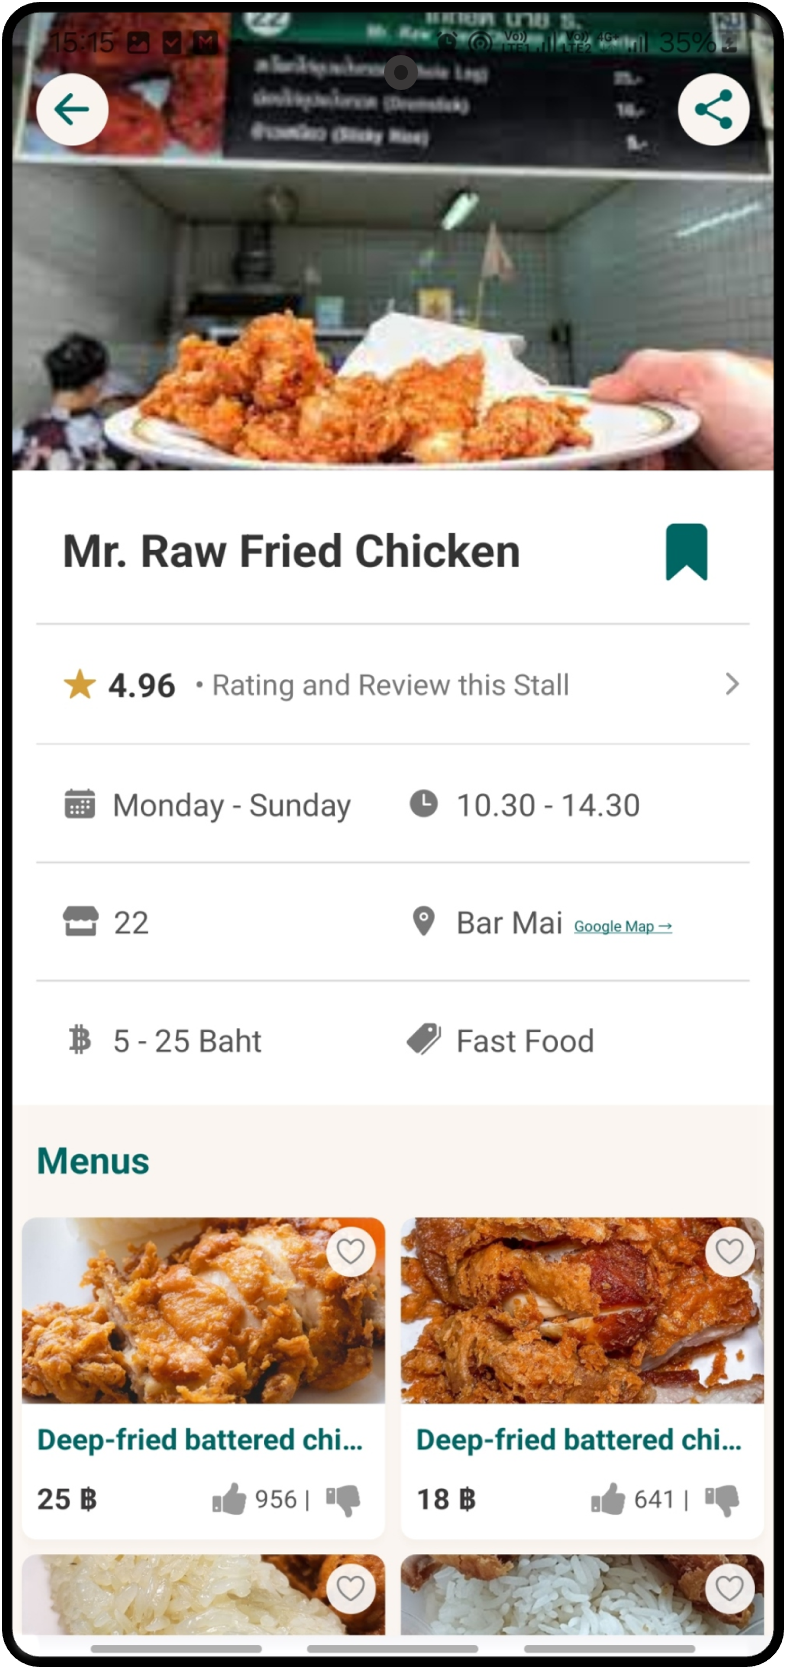
\includegraphics[width=\textwidth,height=0.4\textheight,keepaspectratio]{kueater/screenshots/stall-screen.png}
    \caption{Stall Details}
    \label{fig:stall-screen}
\end{figure}

\begin{figure}[h!]
    \centering
    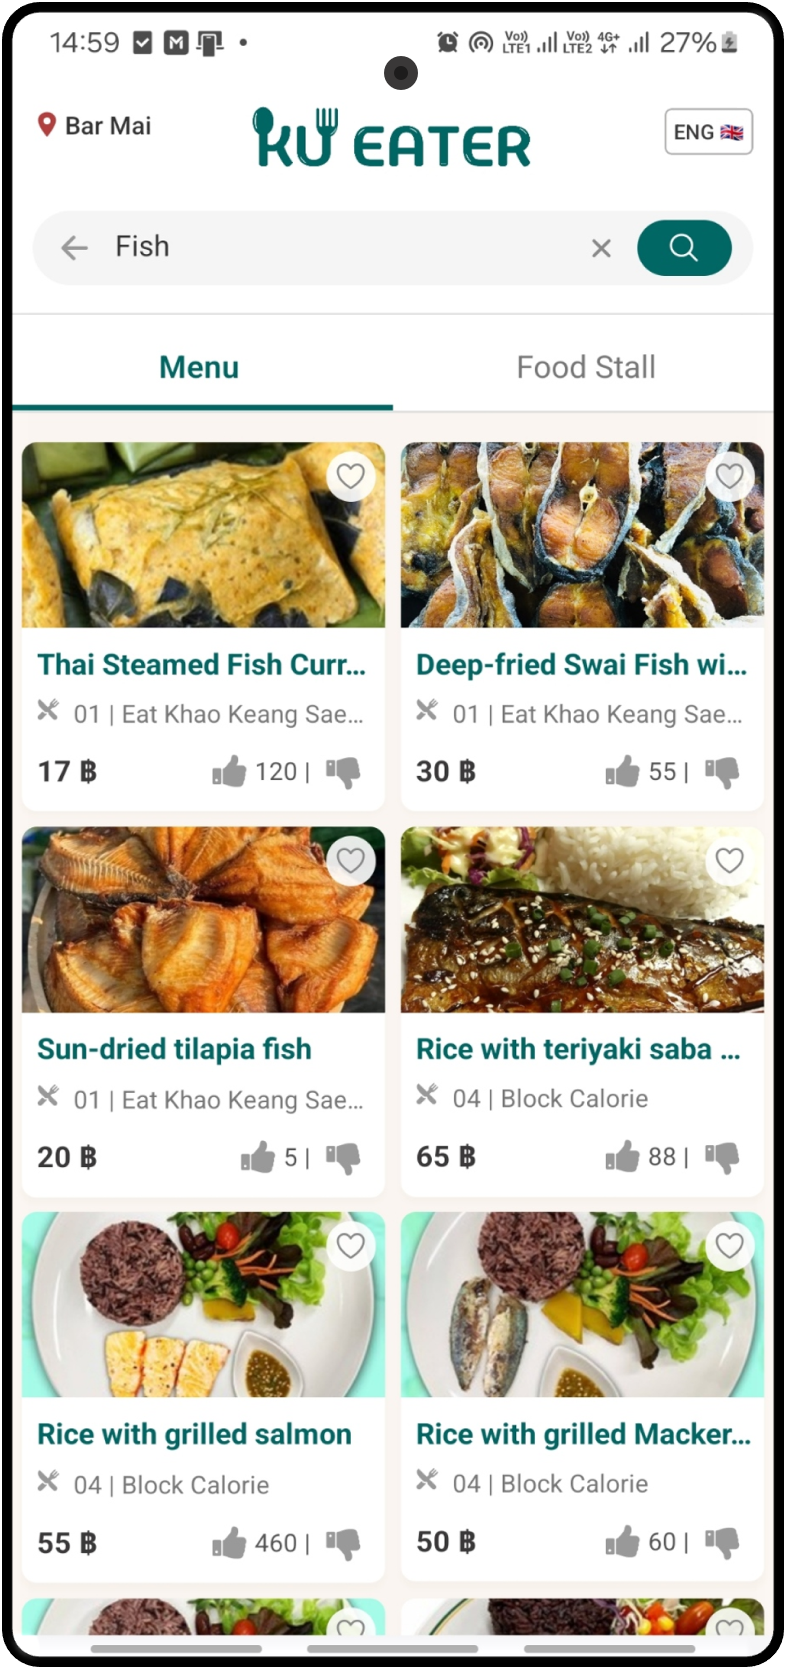
\includegraphics[width=\textwidth,height=0.4\textheight,keepaspectratio]{kueater/screenshots/search-screen.png}
    \caption{Search Page}
    \label{fig:search-screen}
\end{figure}

\begin{figure}[h!]
    \centering
    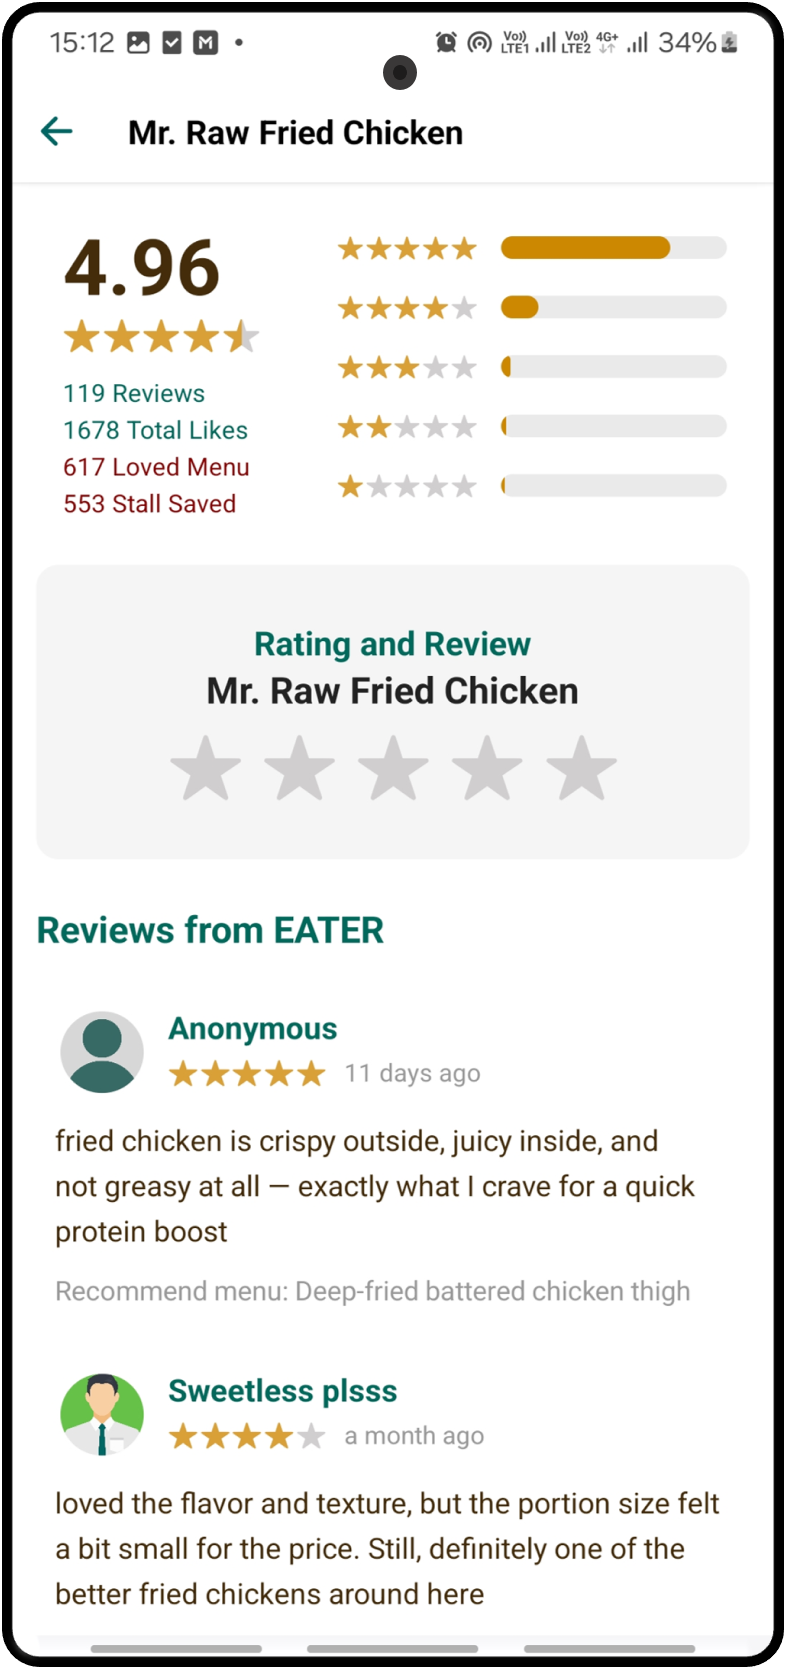
\includegraphics[width=\textwidth,height=0.4\textheight,keepaspectratio]{kueater/screenshots/review.png}
    \caption{Review Screen}
    \label{fig:review-screen}
\end{figure}

\begin{figure}[h!]
    \centering
    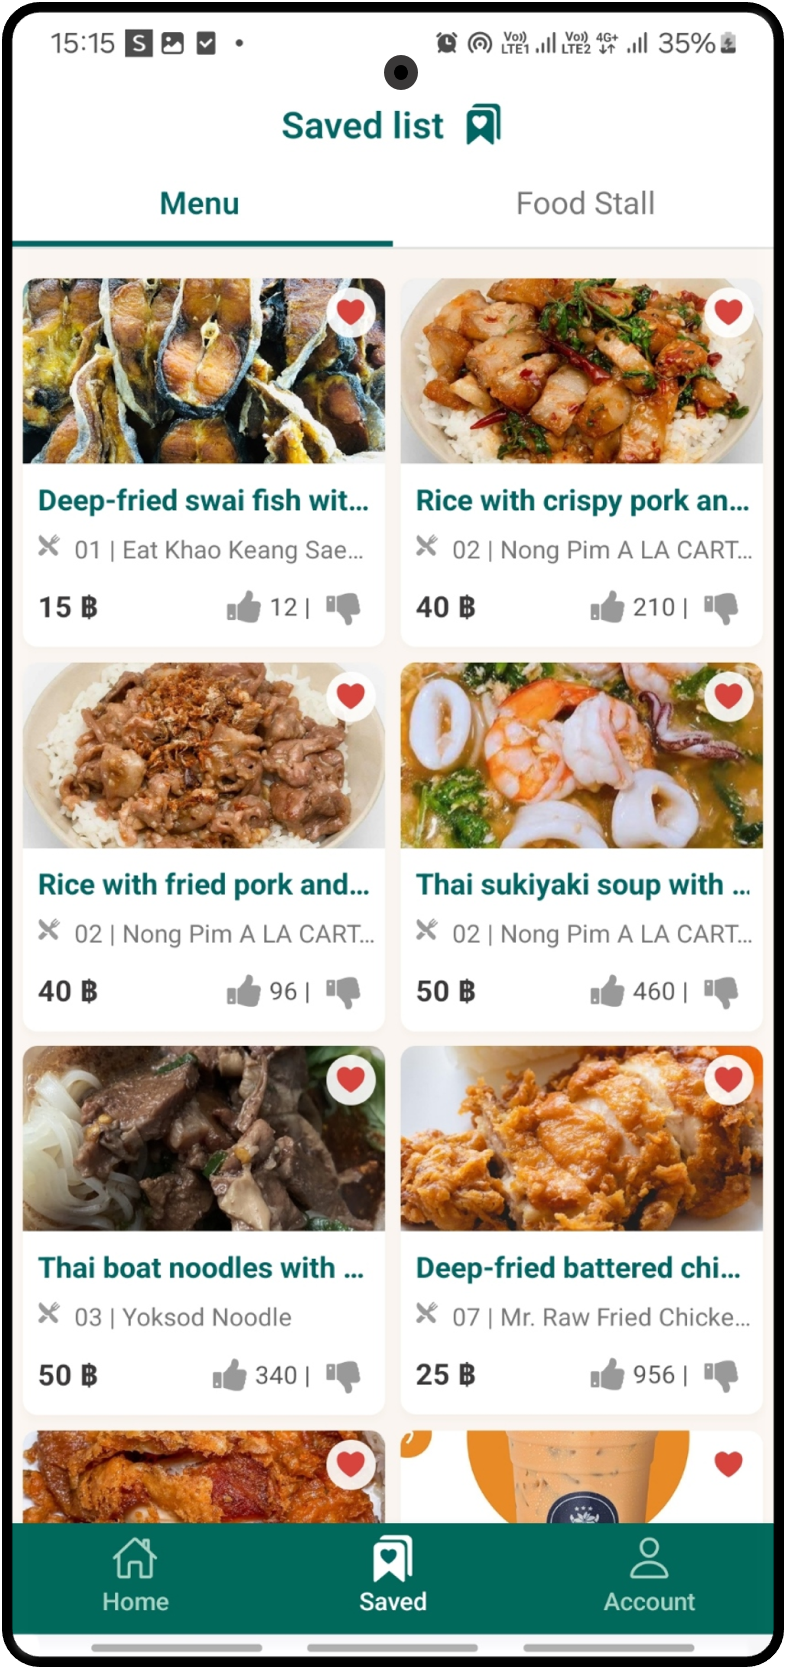
\includegraphics[width=\textwidth,height=0.4\textheight,keepaspectratio]{kueater/screenshots/saved-screen.png}
    \caption{Saved Menu List}
    \label{fig:saved-screen}
\end{figure}


\newappendix{Evaluation Results Charts}

\begin{figure}[h!]
    \centering
    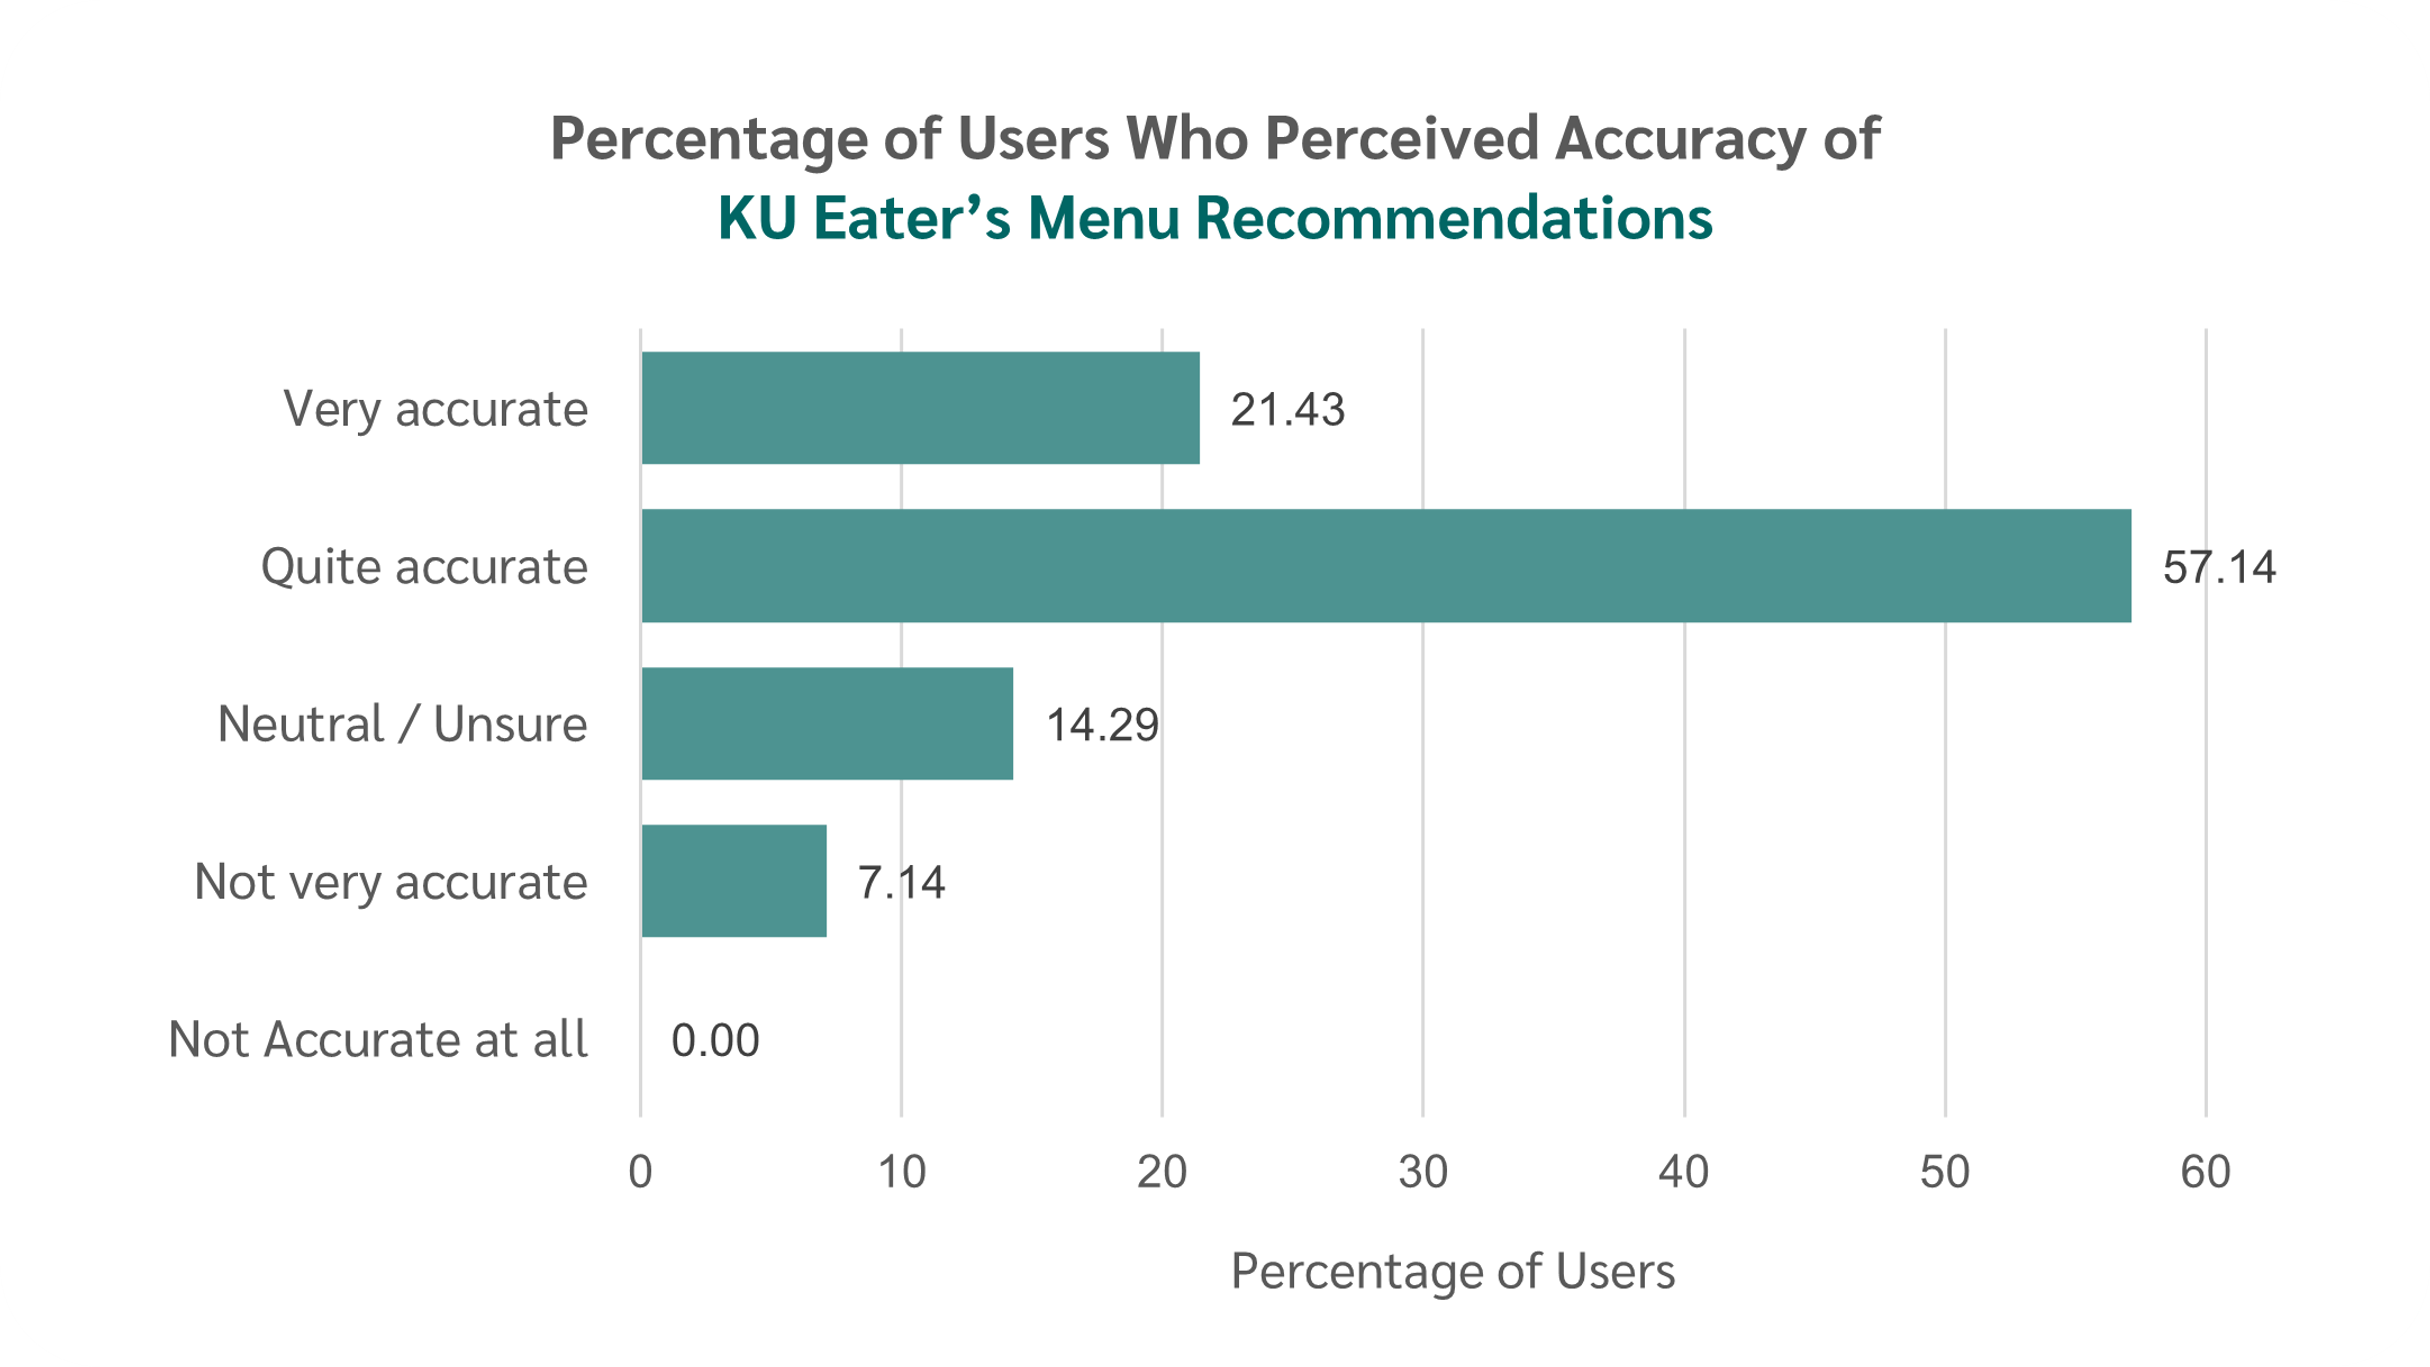
\includegraphics[width=\textwidth,height=0.4\textheight,keepaspectratio]{kueater/recommendation-accuracy.png}
    \caption{Results from Accuracy of Recommendation Evaluation}
    \label{fig:recommendation-accuracy}
\end{figure}

\begin{figure}[h!]
    \centering
    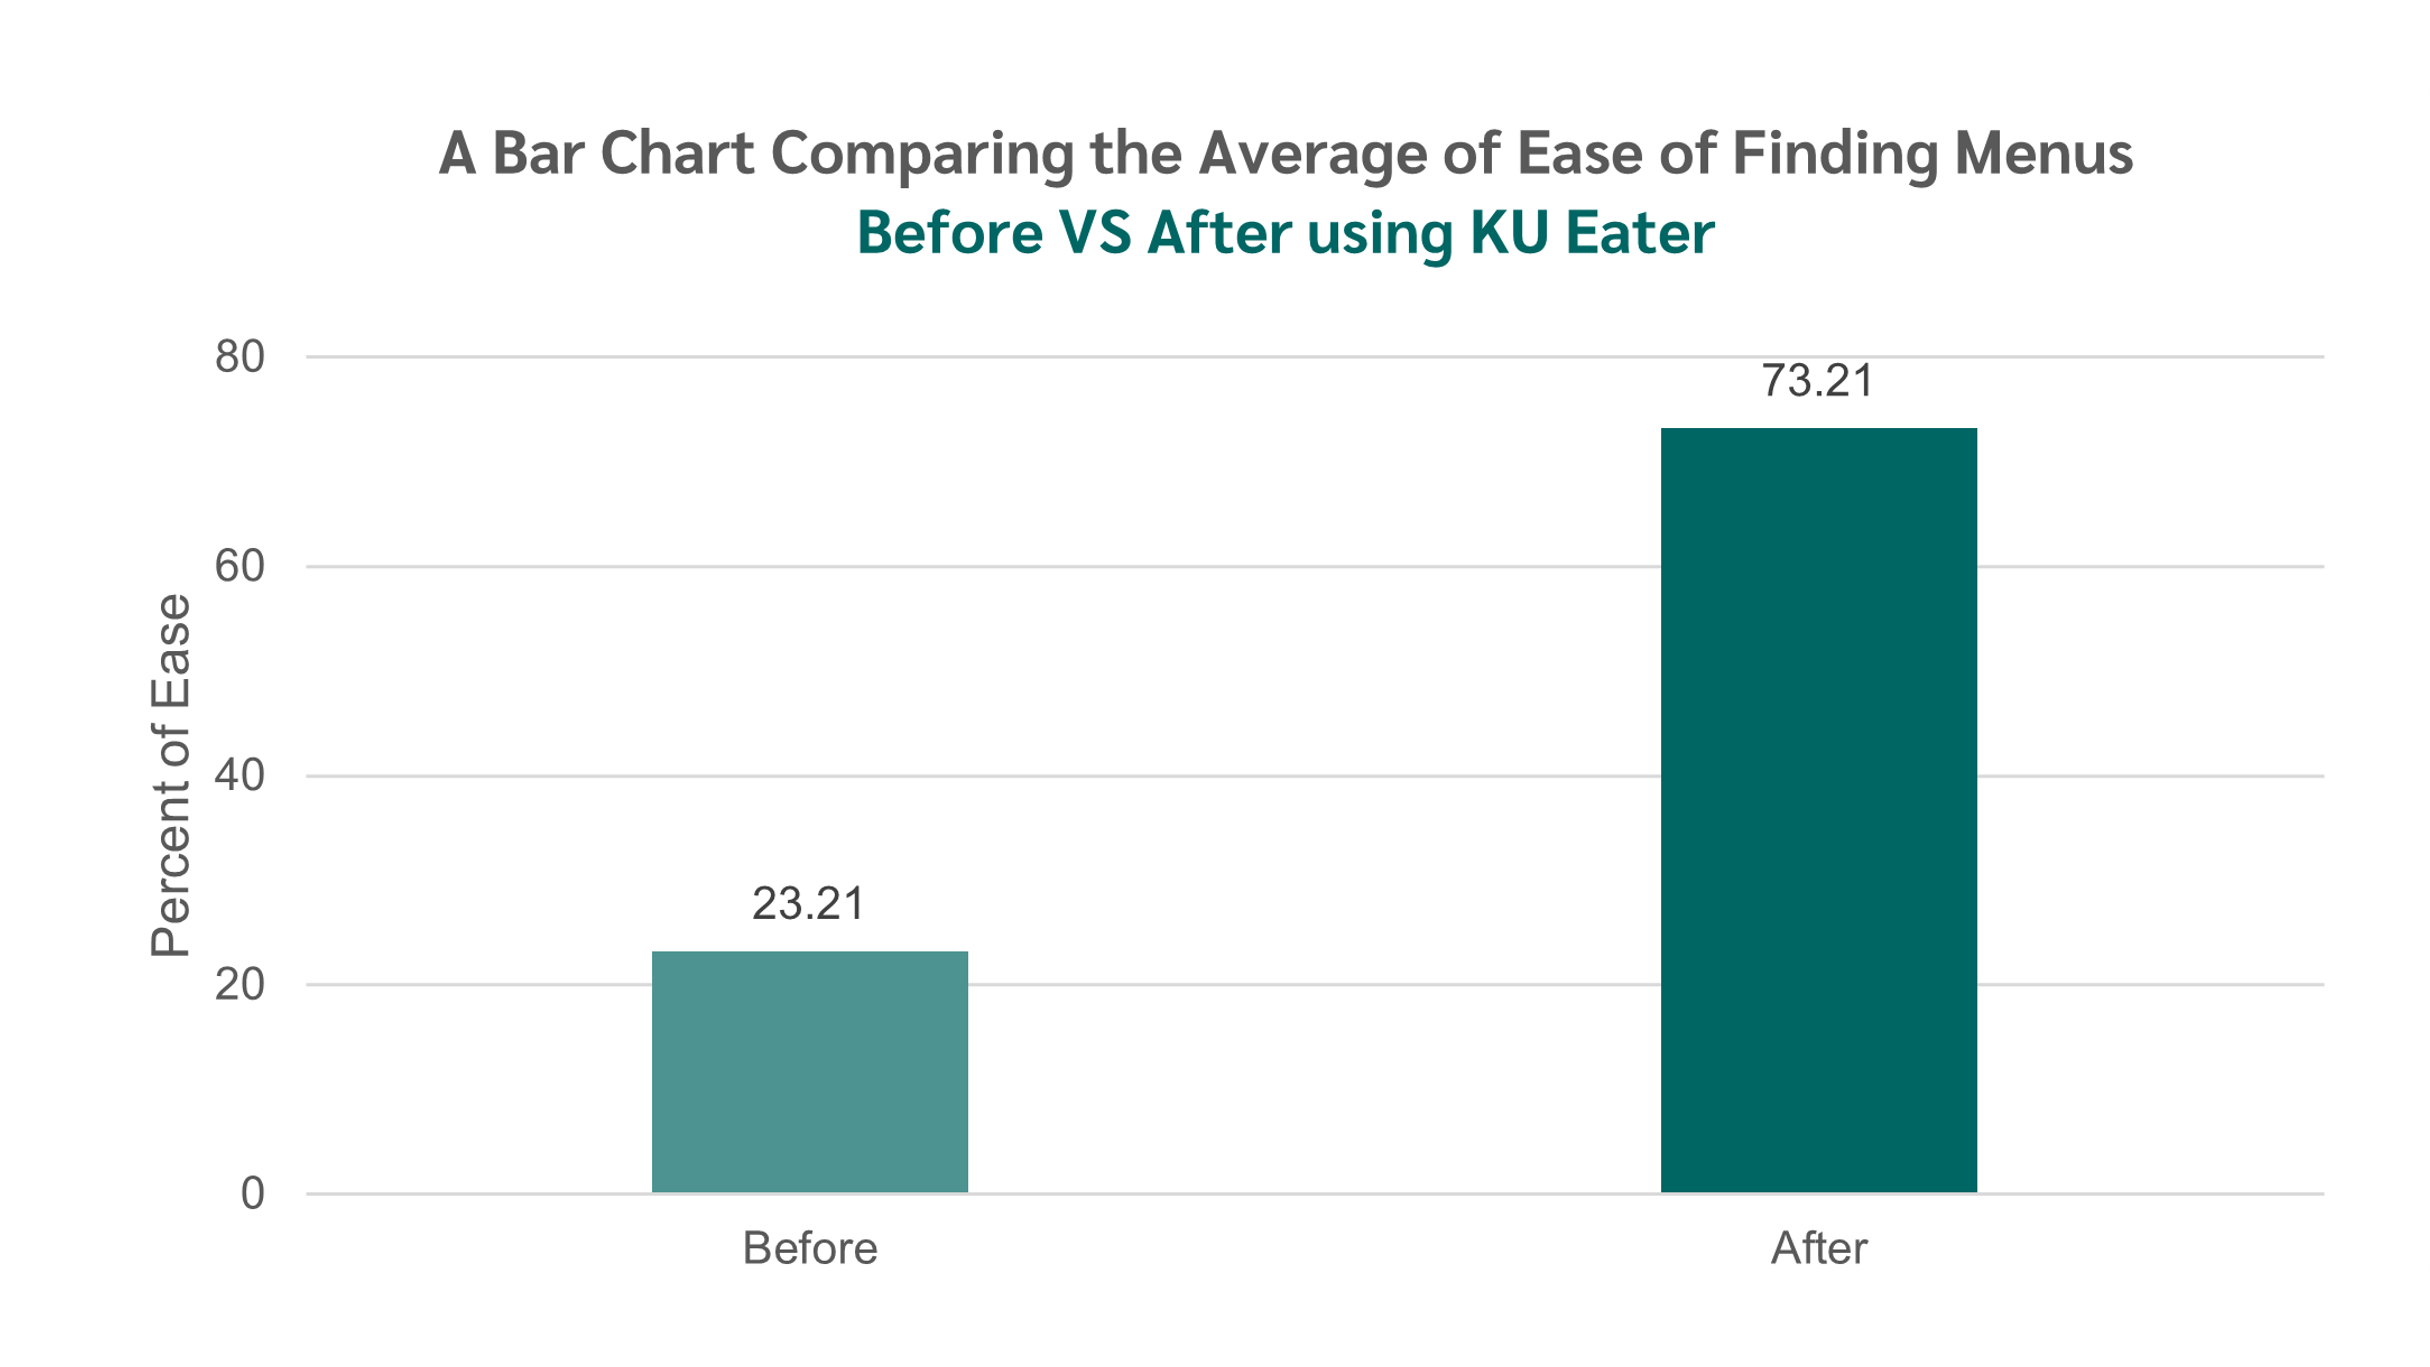
\includegraphics[width=\textwidth,height=0.4\textheight,keepaspectratio]{kueater/ease-of-finding.png}
    \caption{Results from Ease of Finding Food Evaluation}
    \label{fig:ease-of-finding}
\end{figure}

\begin{figure}[h!]
    \centering
    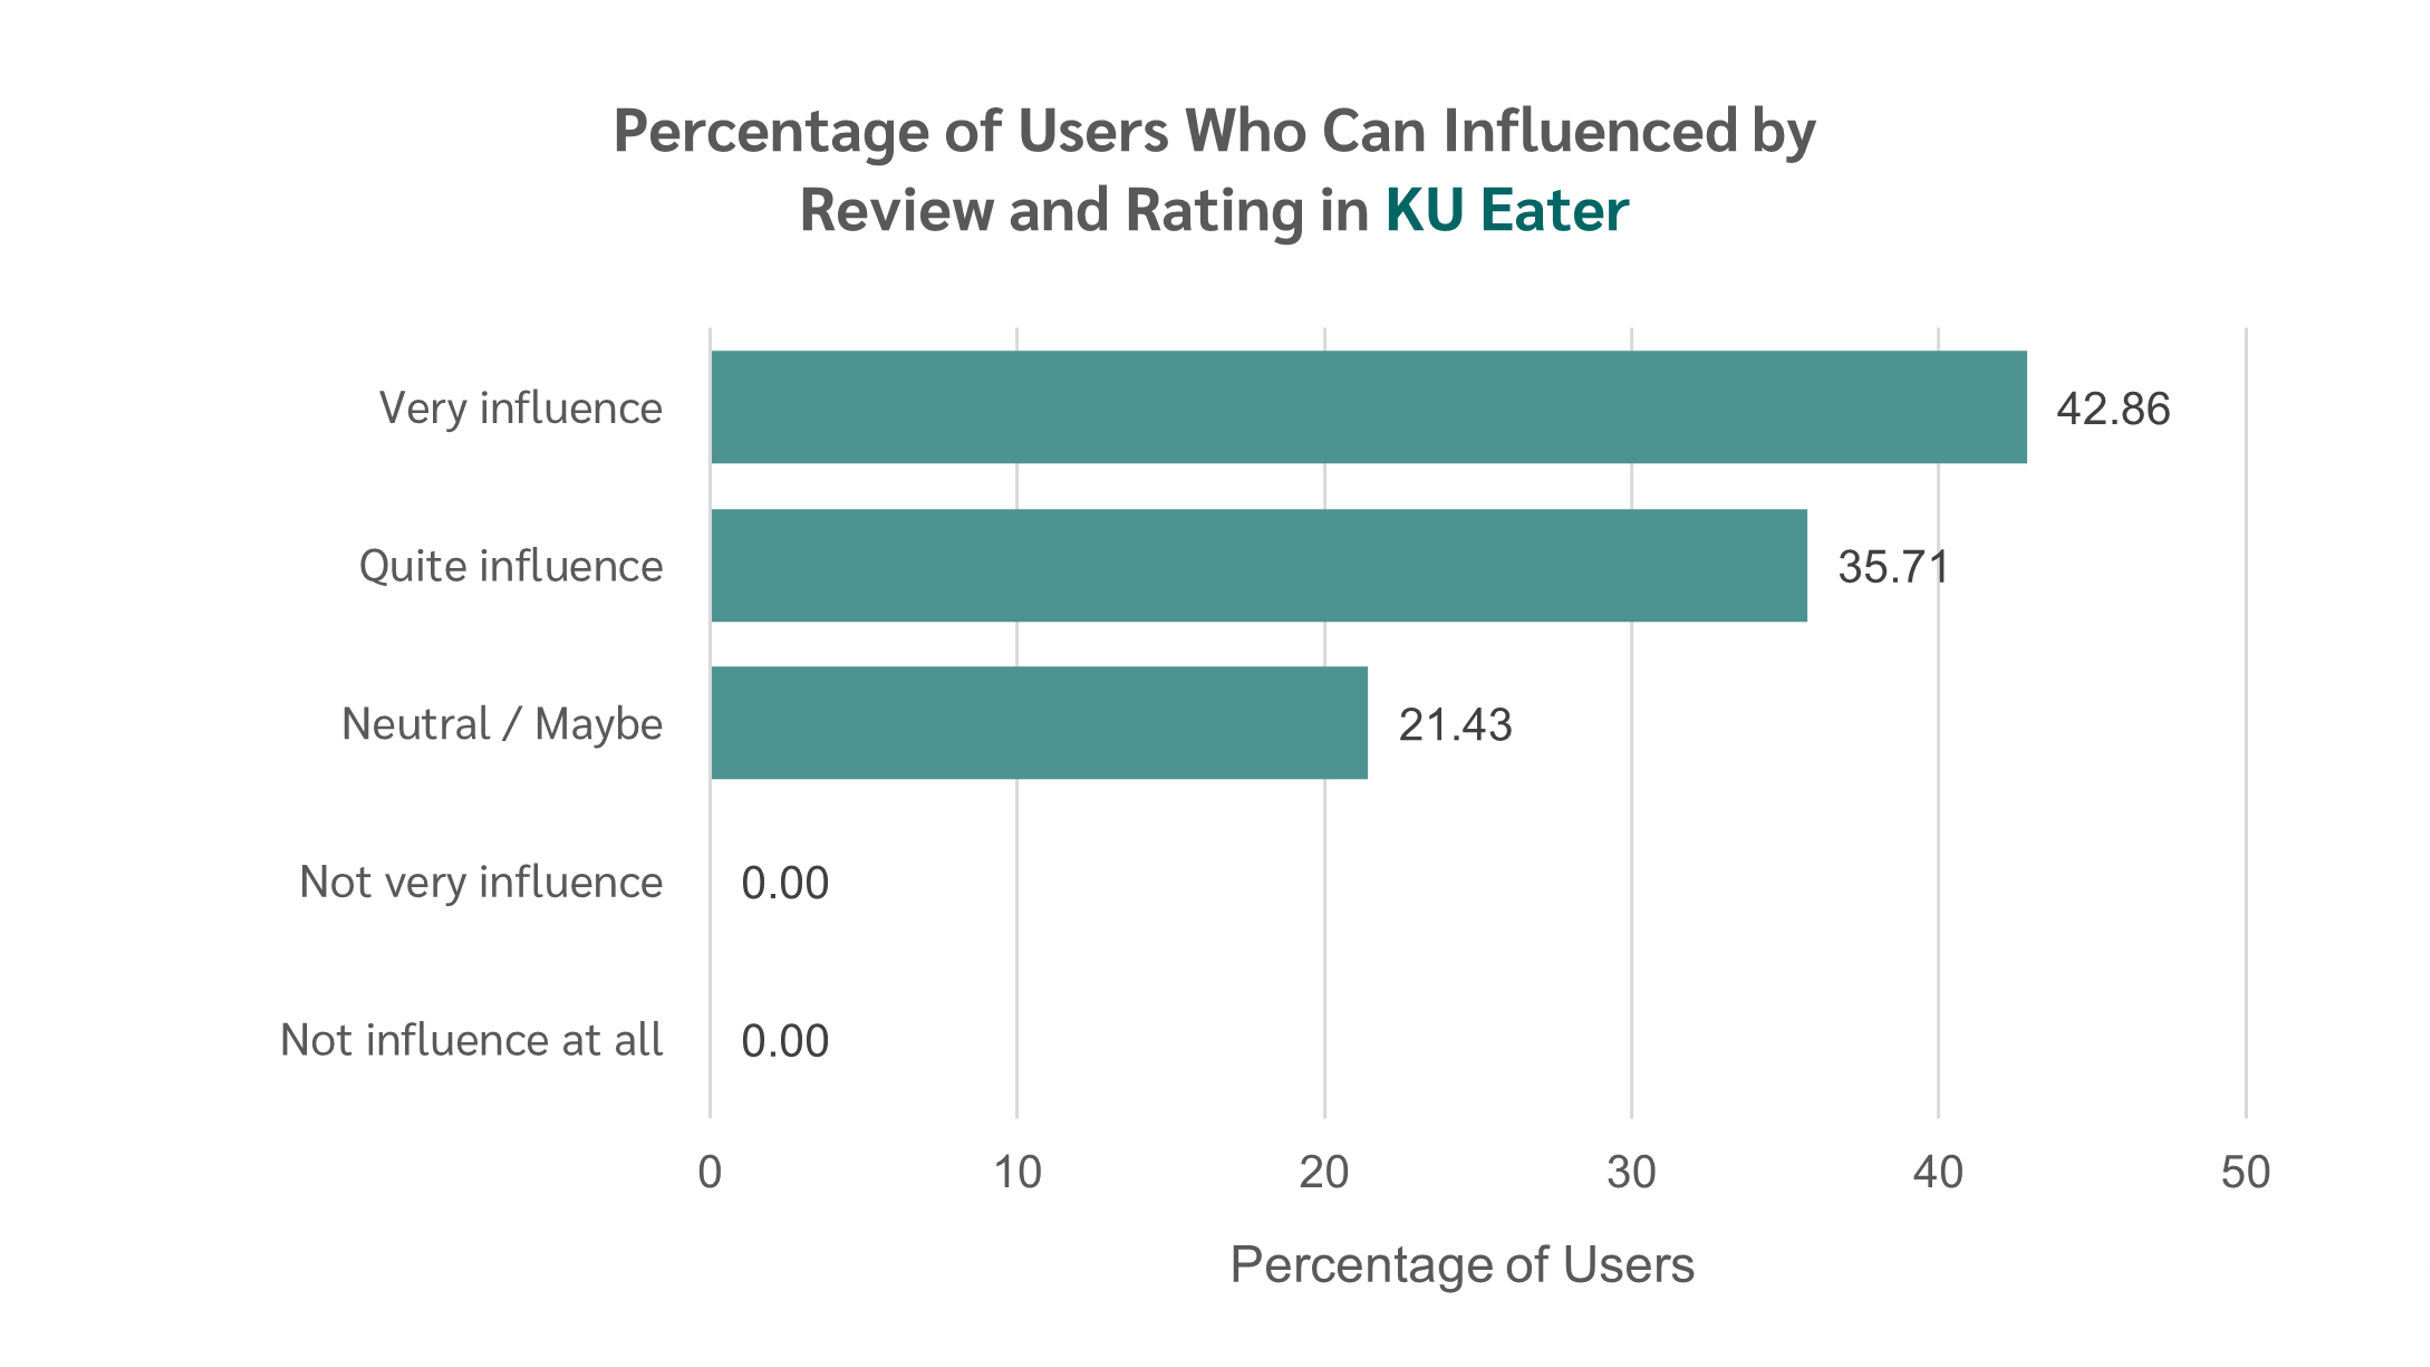
\includegraphics[width=\textwidth,height=0.4\textheight,keepaspectratio]{kueater/influenced-by-review.png}
    \caption{Results from How Reviews Influenced Users}
    \label{fig:influenced-by-review}
\end{figure}

\begin{figure}[h!]
    \centering
    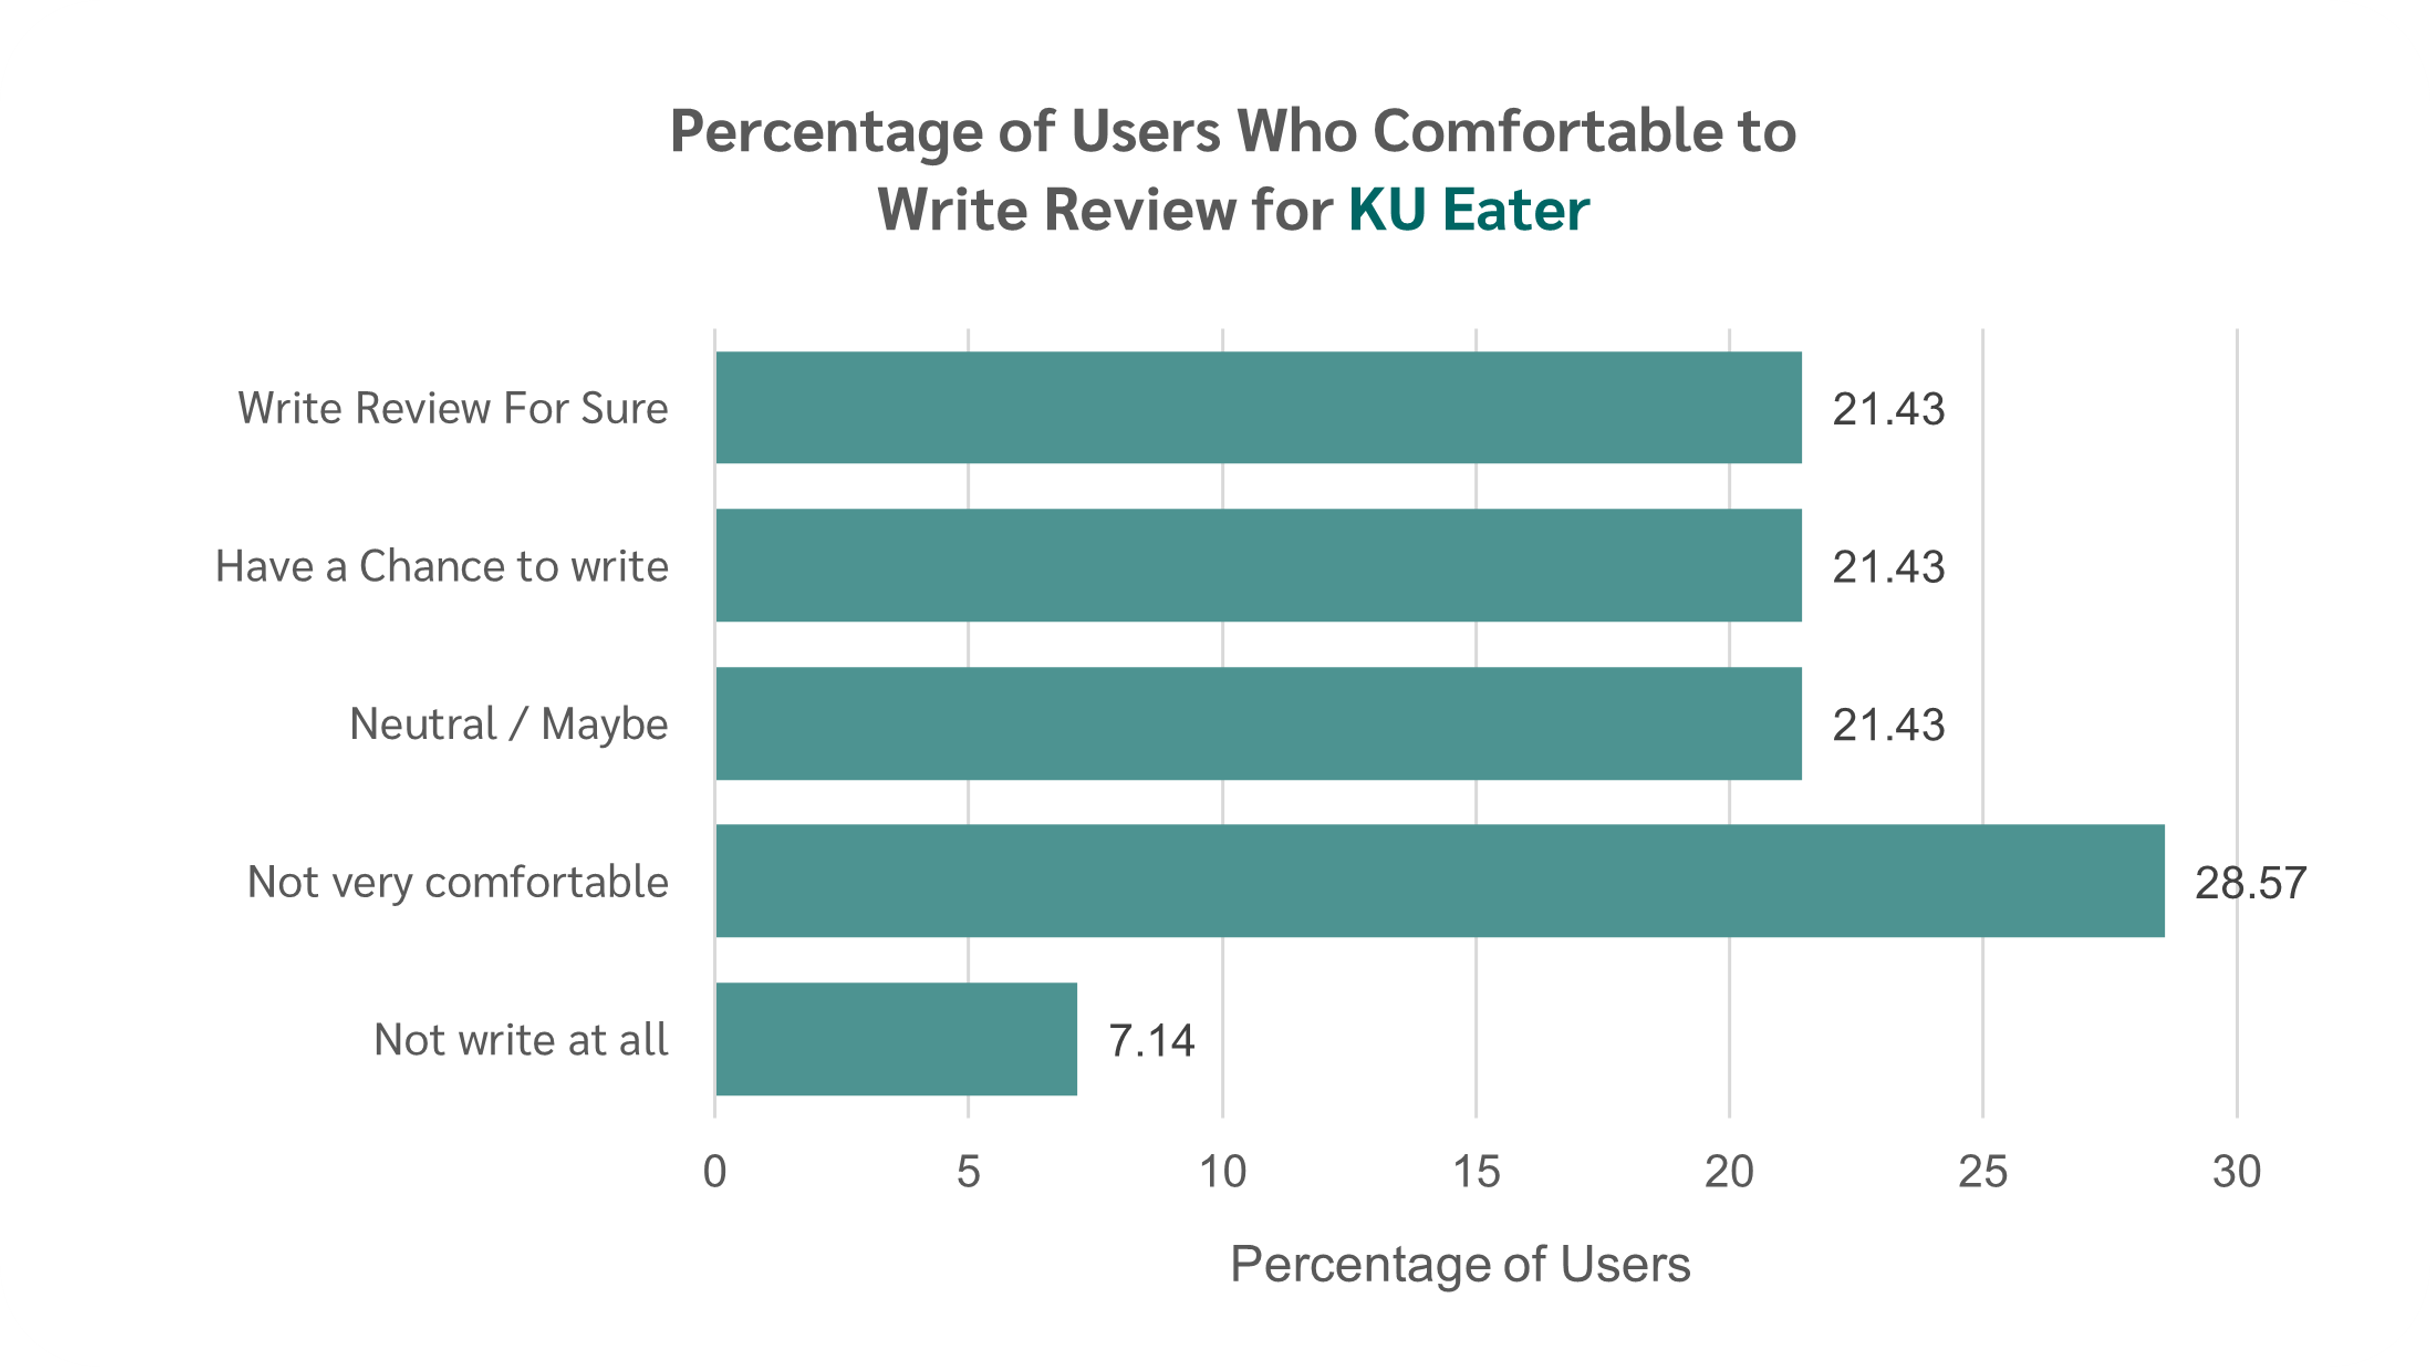
\includegraphics[width=\textwidth,height=0.4\textheight,keepaspectratio]{kueater/likelihood-to-write.png}
    \caption{Results from Likelihood to Write Reviews}
    \label{fig:likelihood-to-write}
\end{figure}

\begin{figure}[h!]
    \centering
    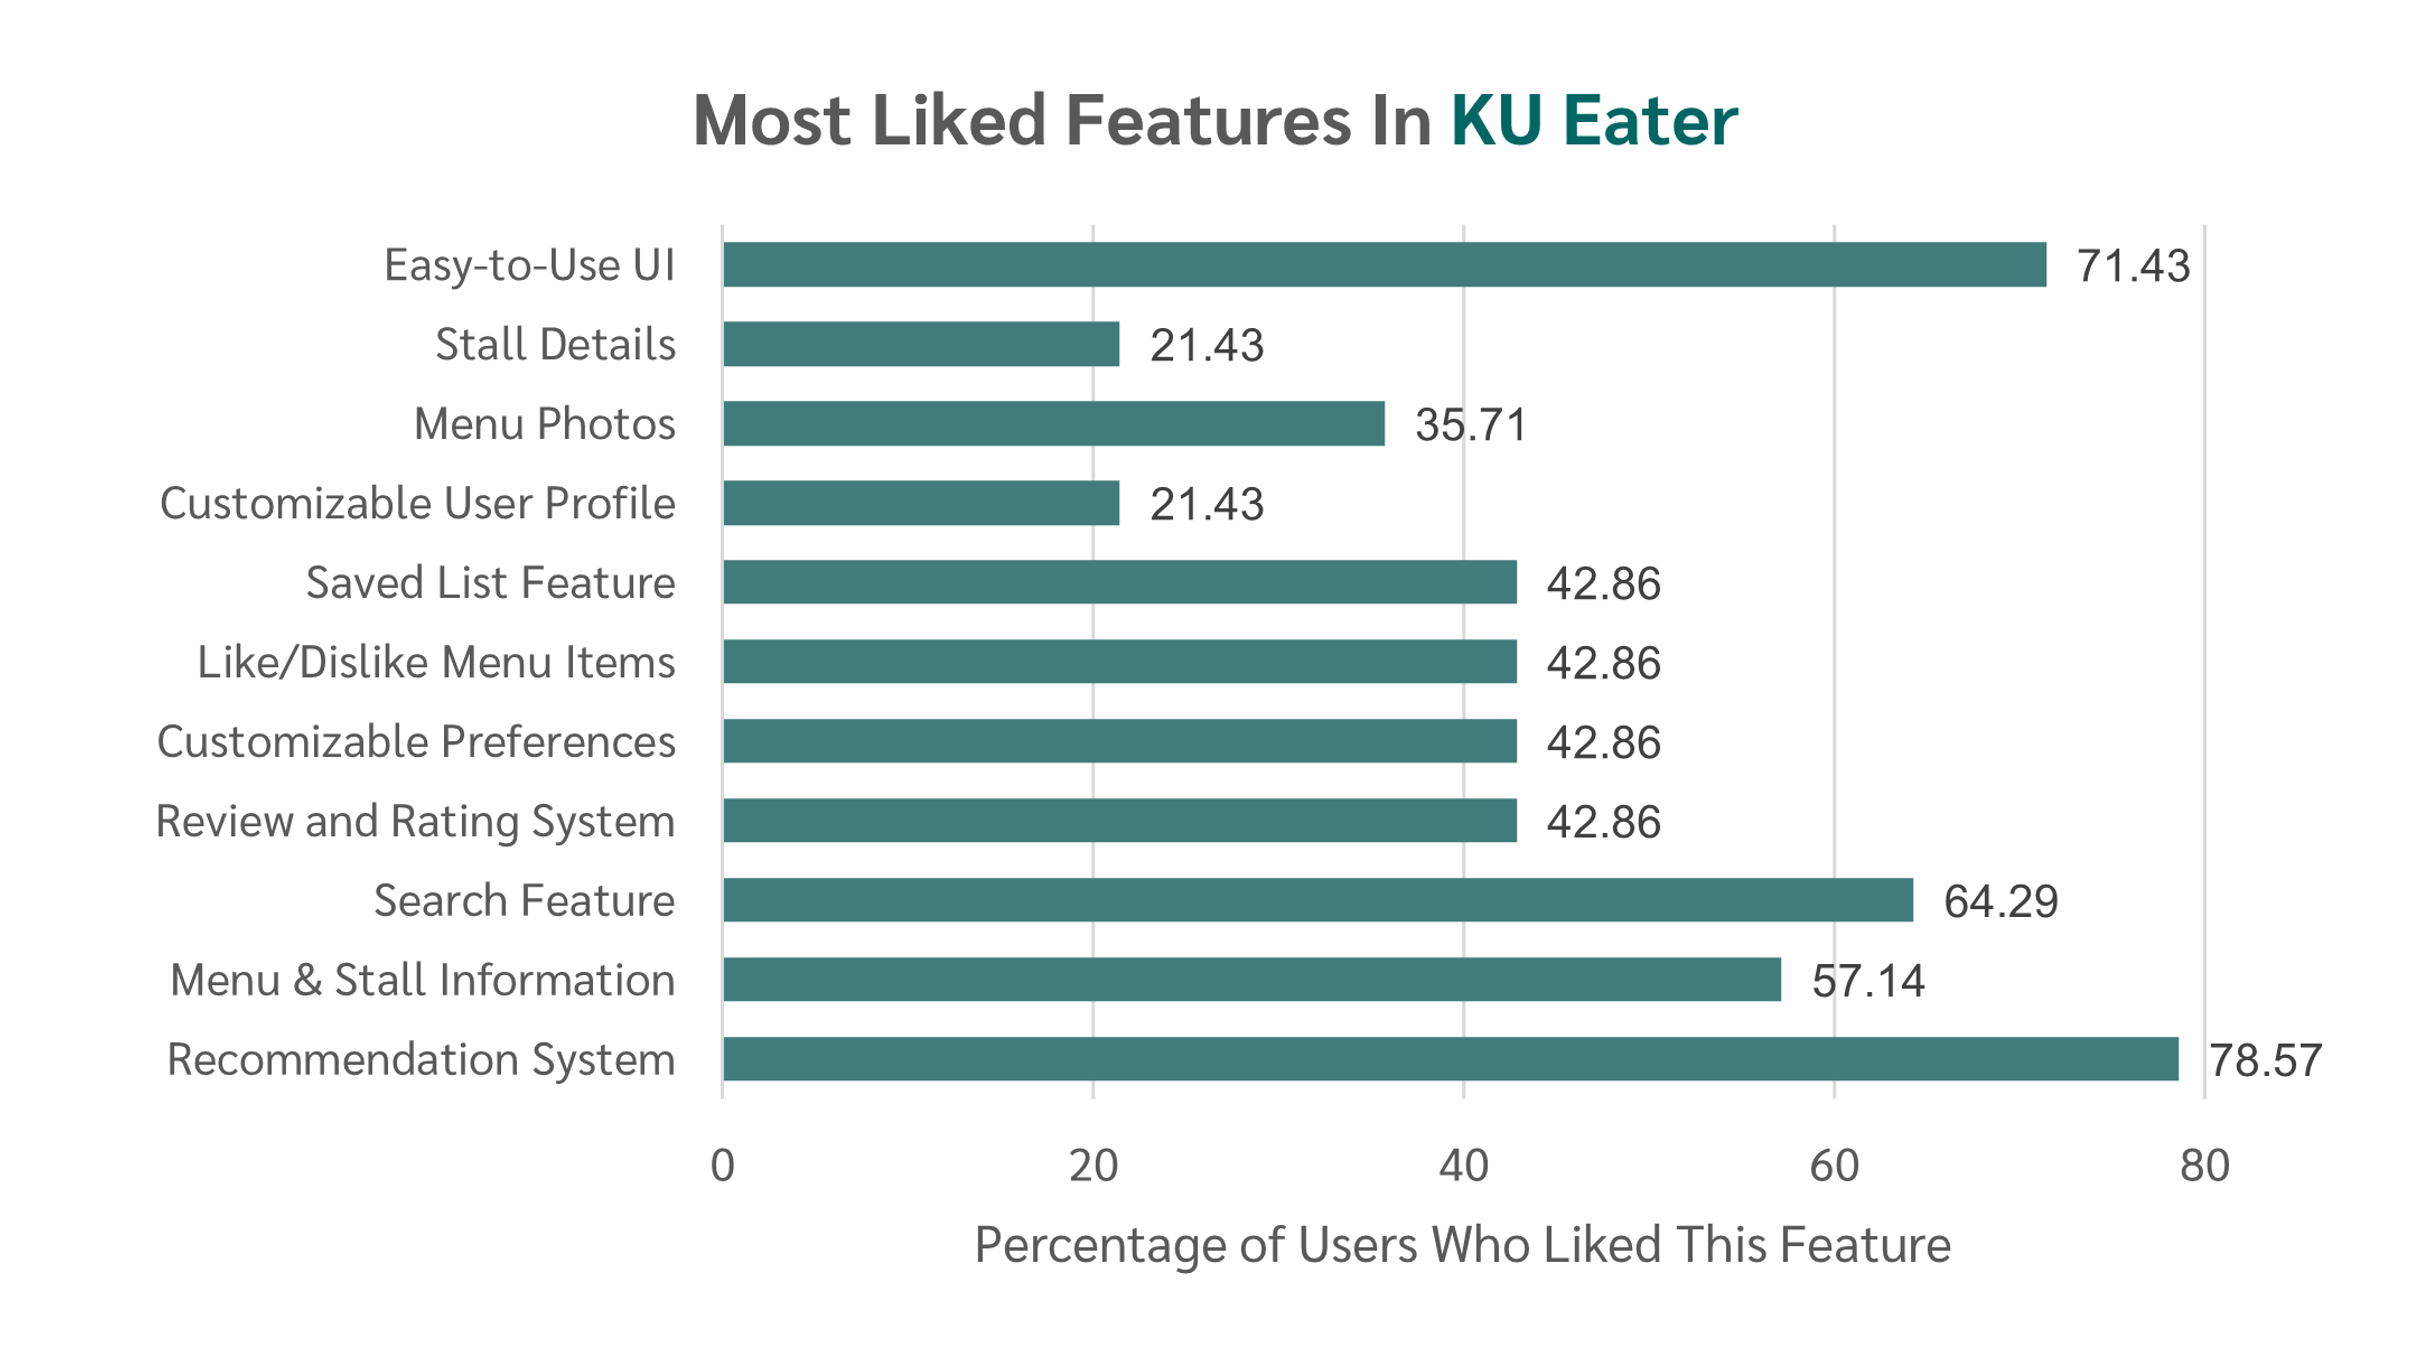
\includegraphics[width=\textwidth,height=0.4\textheight,keepaspectratio]{kueater/most-liked-features.png}
    \caption{Most Liked Feature by User Evaluation}
    \label{fig:most-liked-features}
\end{figure}

\begin{figure}[h!]
    \centering
    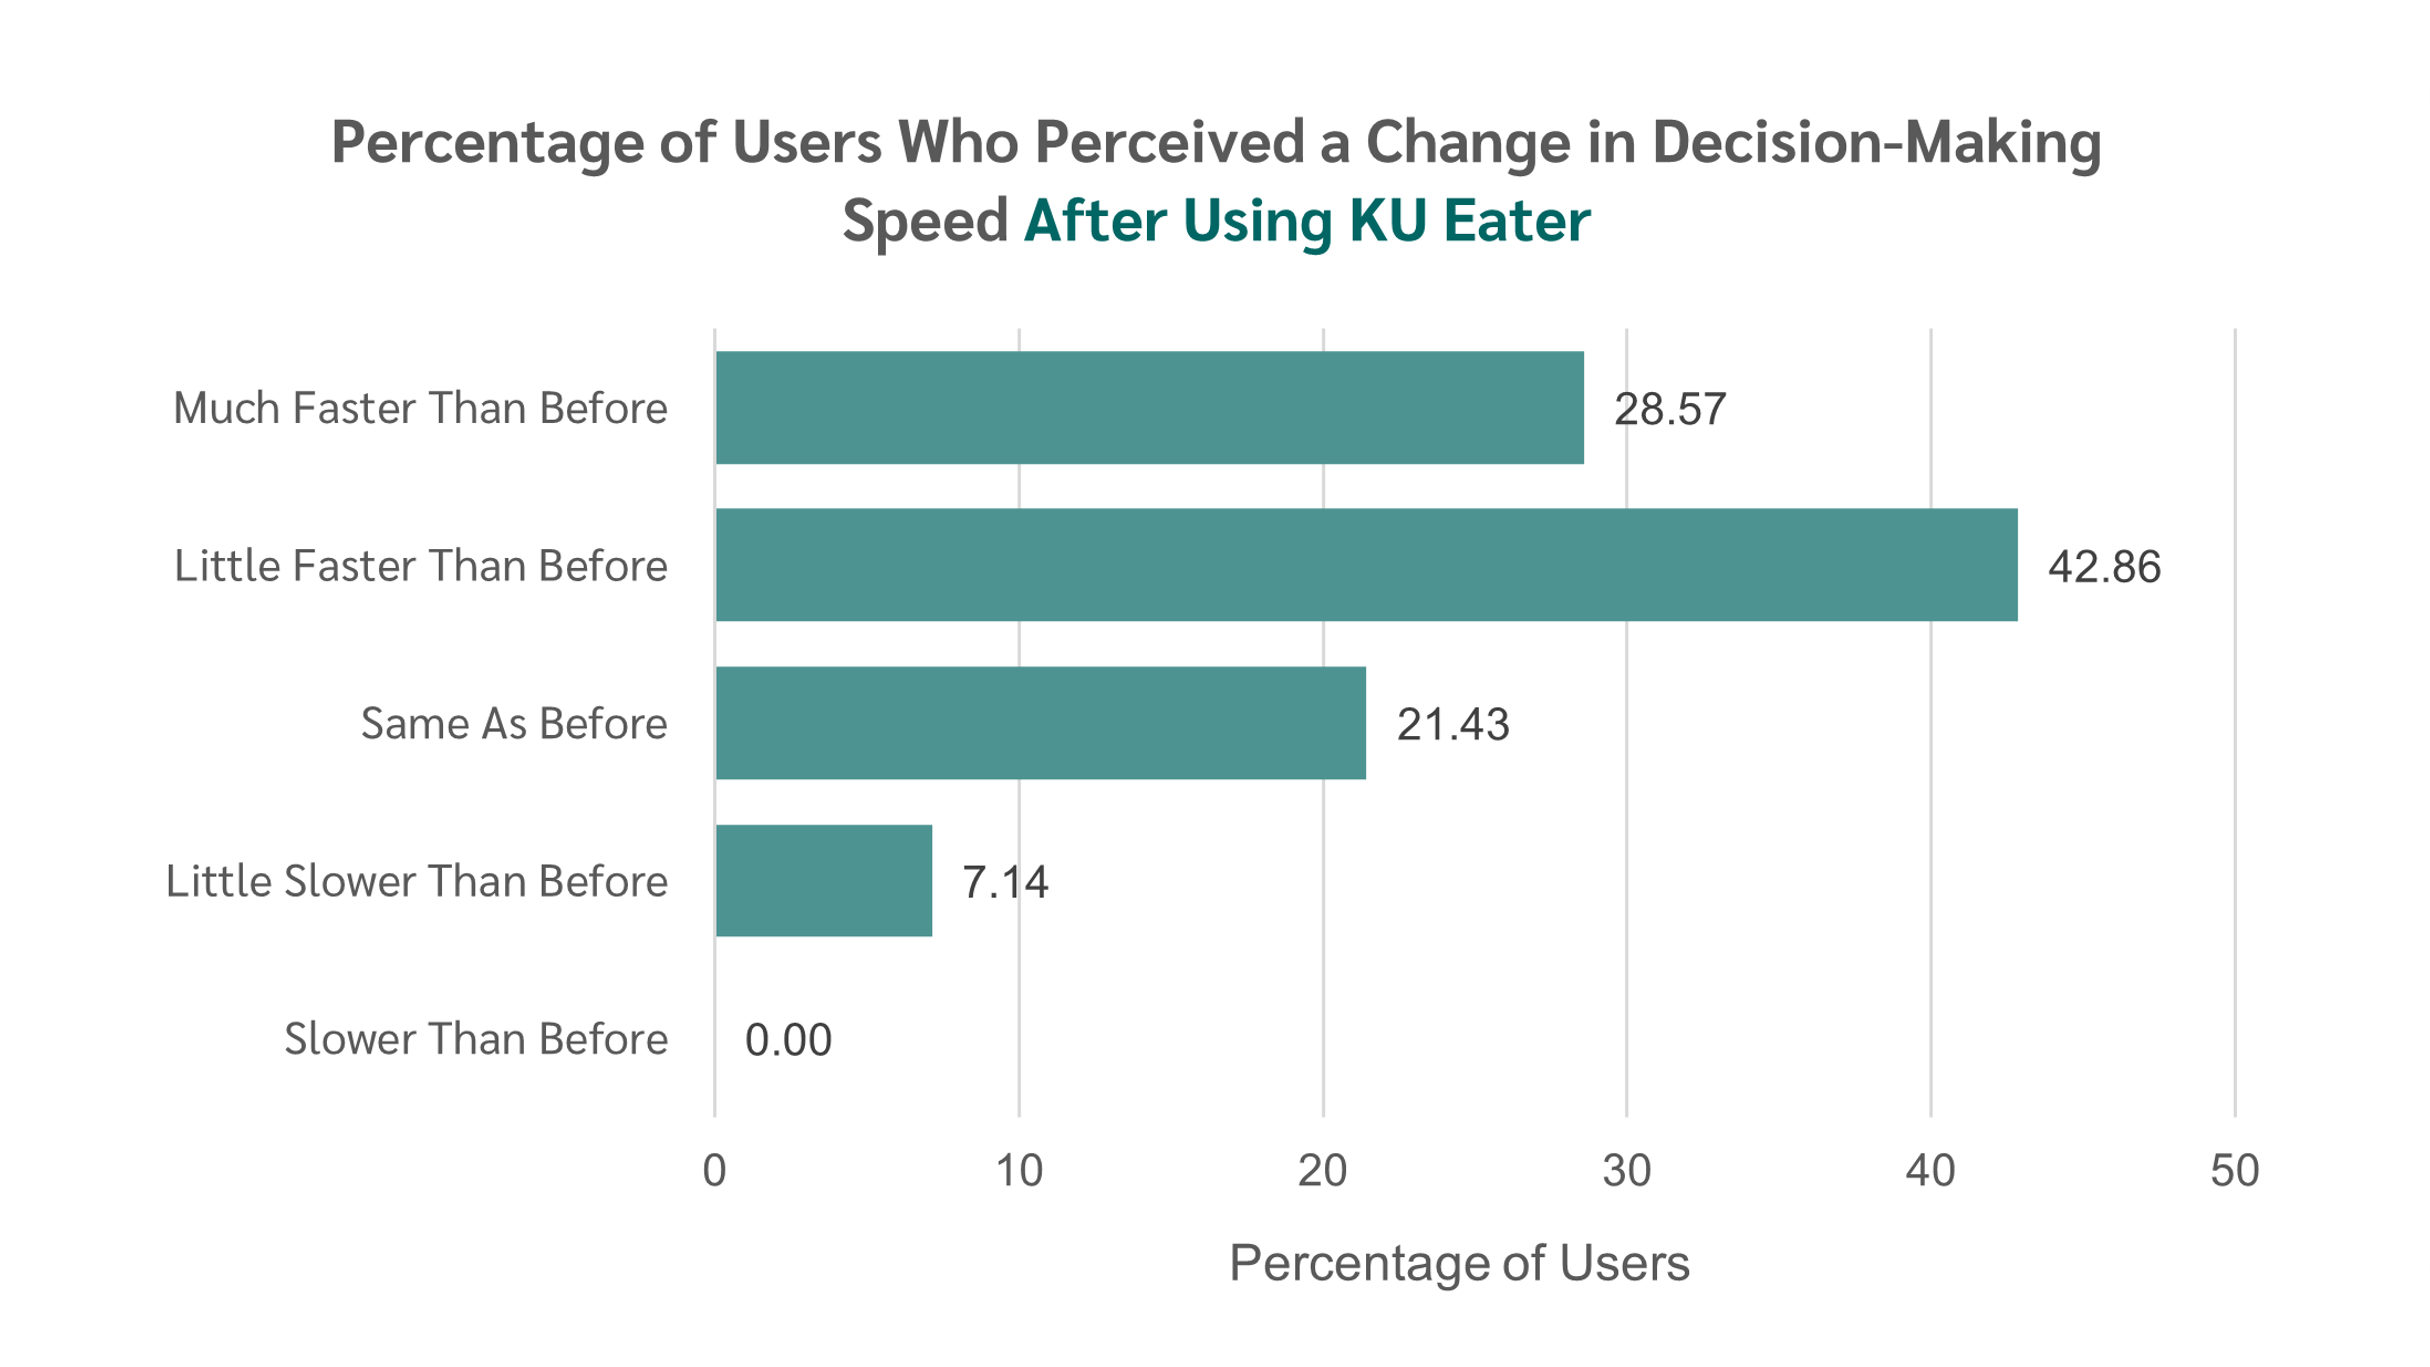
\includegraphics[width=\textwidth,height=0.4\textheight,keepaspectratio]{kueater/decision-making-speed.png}
    \caption{Results from Users' Decision Making Process}
    \label{fig:decision-making-speed}
\end{figure}

\begin{figure}[h!]
    \centering
    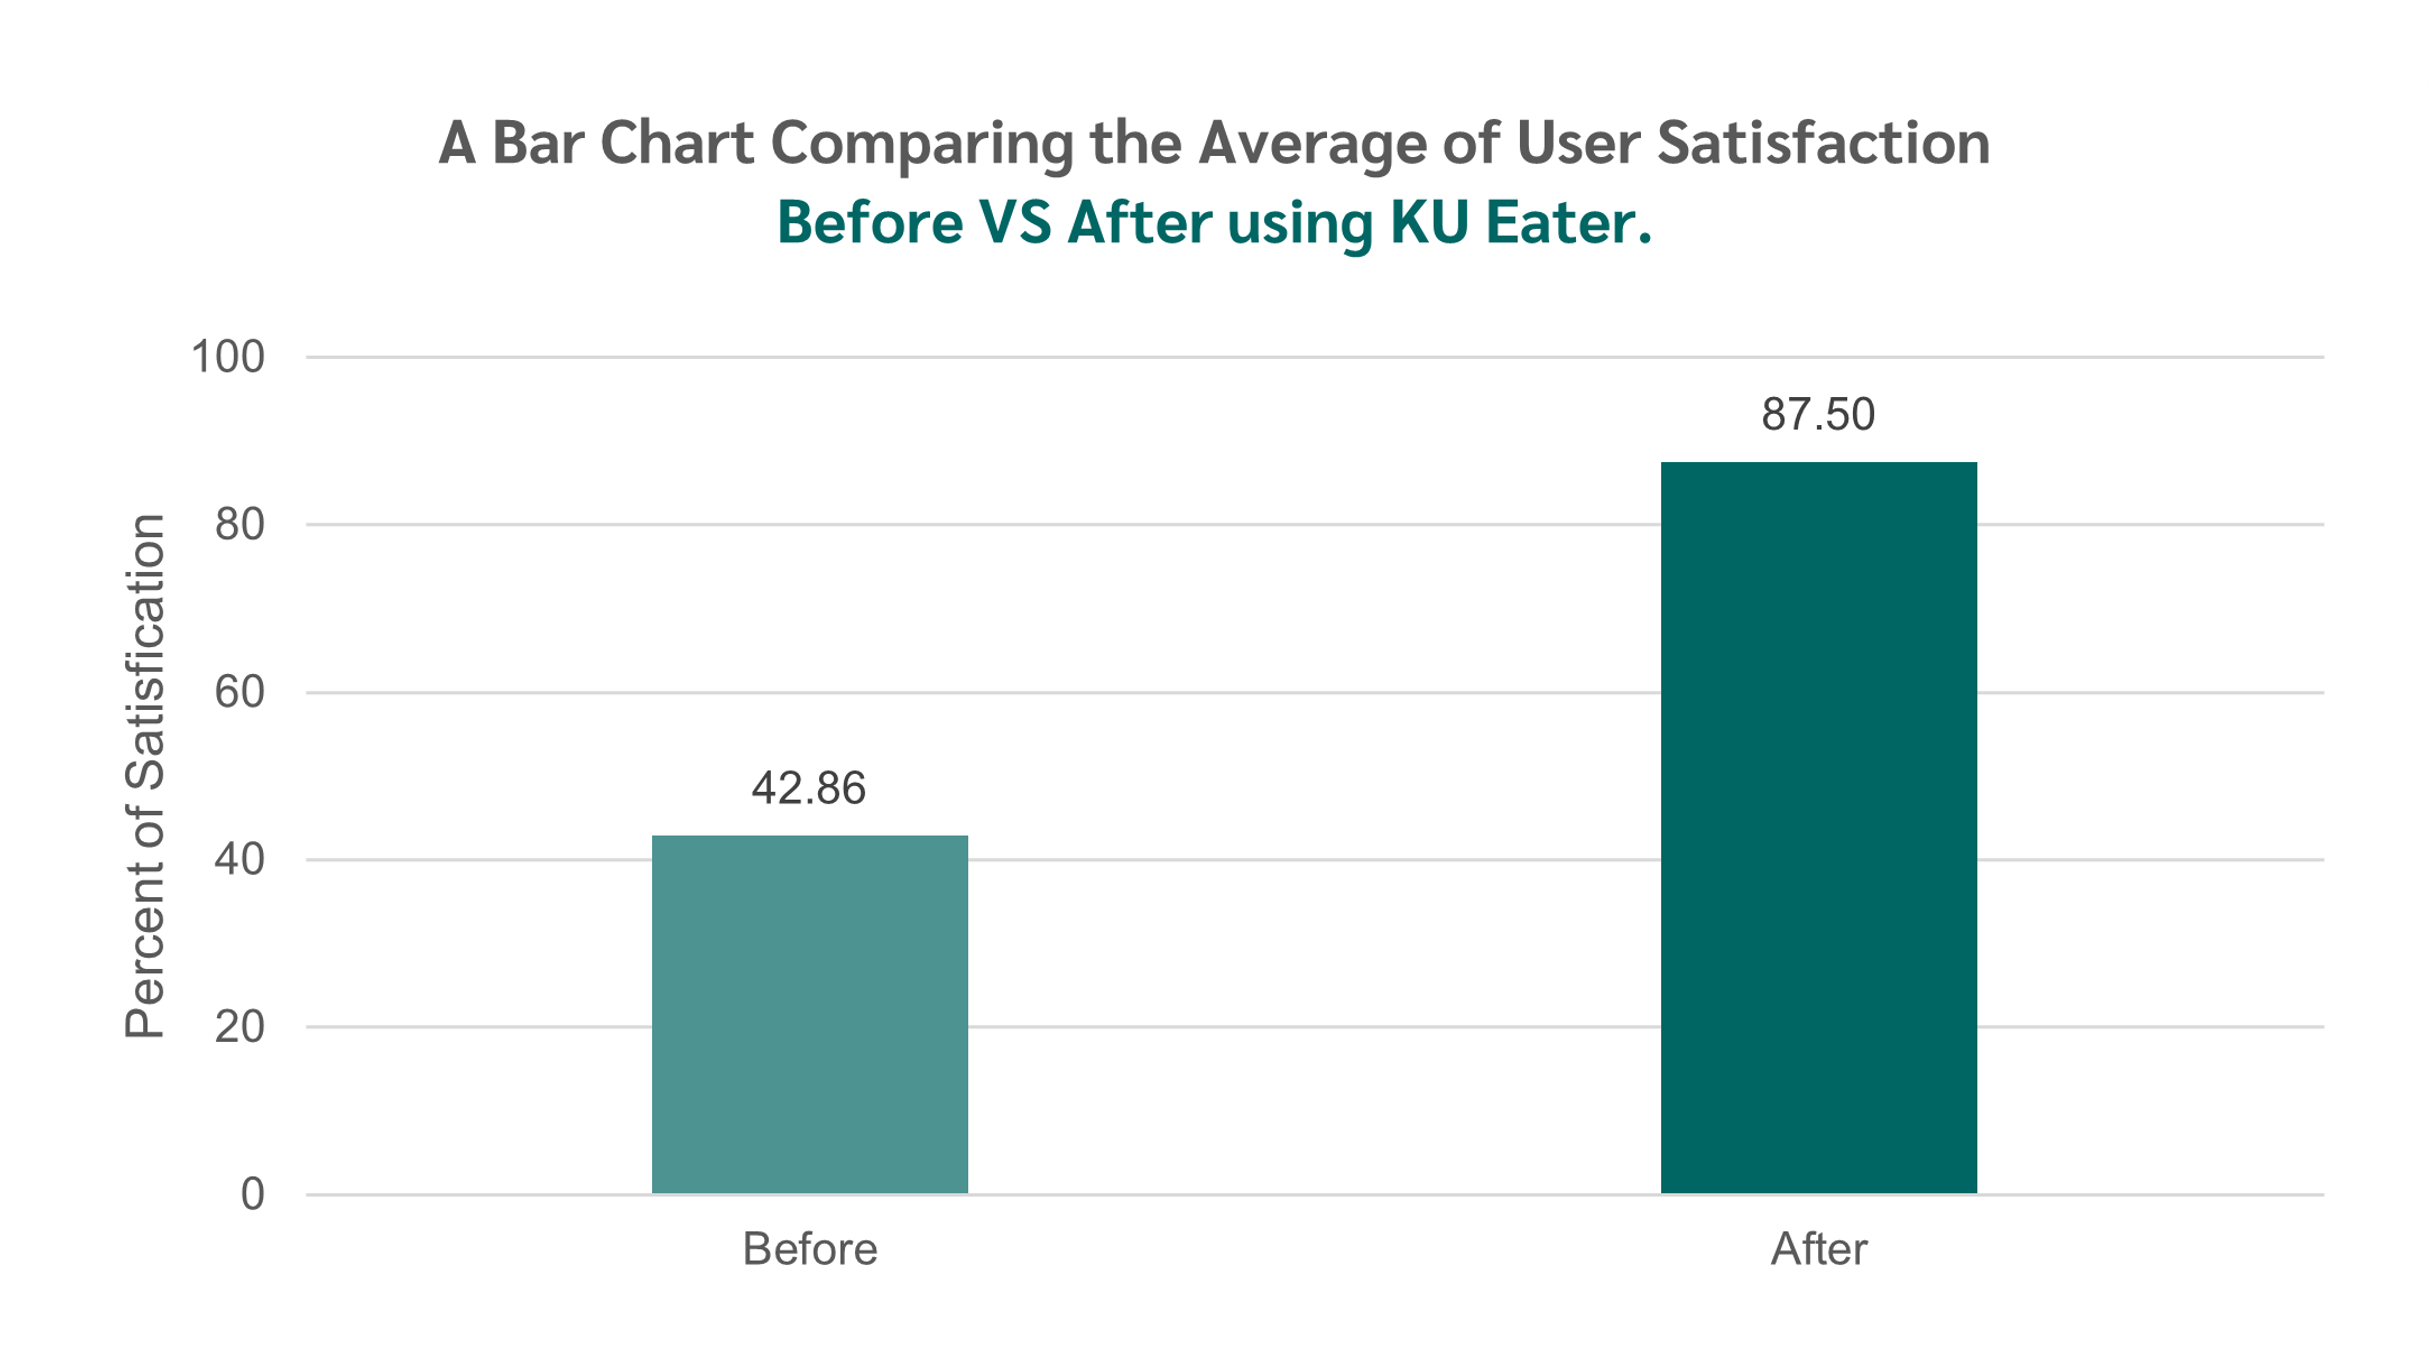
\includegraphics[width=\textwidth,height=0.4\textheight,keepaspectratio]{kueater/overall-satisfaction.png}
    \caption{Overall Statisfaction}
    \label{fig:overall-satisfaction}
\end{figure}